\newpage
\subsection{QuizziPedia::Front-End::QML}


\begin{figure} [ht]
	\centering
	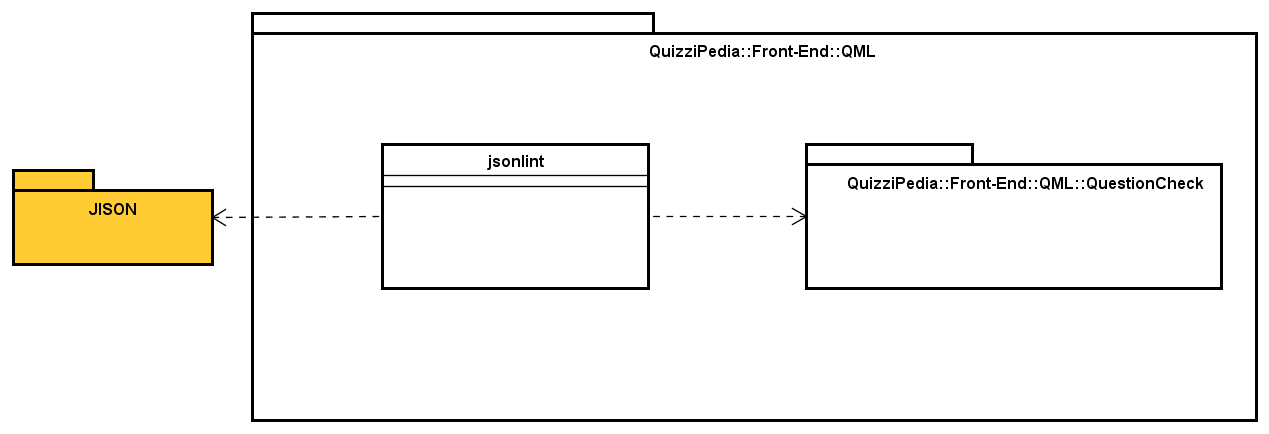
\includegraphics[scale=0.42]{UML/Package/QuizziPedia_Front-End_QML.png}
	\caption{QuizziPedia::Front-End::QML}
\end{figure} \FloatBarrier

\subsubsection{Informazioni generali}
\begin{itemize}
	\item \textbf{Descrizione}: \textit{package\ped{G}} che contiene i componenti individuati per la parte realizzazione del linguaggio di \textit{markup\ped{G}} \textit{QML\ped{G}} dell'applicazione;
	\item \textbf{Padre}: \texttt{Front-End};
	\item \textbf{Interazione con altri componenti}:
	\begin{itemize}
		\item \texttt{Controller}: \textit{package\ped{G}} che contiene le classi controller individuate;
		\item \texttt{View}: \textit{package\ped{G}} che contiene le classi view individuate.
	\end{itemize} 
\end{itemize}
\subsubsection{Classi}

\paragraph[QuizziPedia::Front-End::QML::jsonlint]{QuizziPedia::Front-End::QML::jsonlint}
\begin{figure} [ht]
	\centering
	\includegraphics[scale=0.80]{UML/Classi/Front-End/QuizziPedia_Front-end_QML_jsonlint.png}
	\caption{QuizziPedia::Front-End::QML::jsonlint}
\end{figure} \FloatBarrier
\begin{itemize}
	\item \textbf{Descrizione}: questa classe implementa il \textit{parser\ped{G}} per il controllo della grammatica del \textit{QML\ped{G}};
	\item \textbf{Utilizzo}: fornisce le funzionalità per controllare la validità sintattica del codice \textit{QML\ped{G}};
	\item \textbf{Relazioni con altre classi}:
	\begin{itemize}
		\item \textbf{IN} \texttt{EditorQMLview}: \textit{view\ped{G}} contenente l'\textit{editor\ped{G}} \textit{QML\ped{G}} per la creazione di domande personalizzate,
		permette ad un utente di creare domande personalizzate attraverso la scrittura del codice \textit{QML\ped{G}} direttamente nell'\textit{editor\ped{G}} di testo presente nella \textit{view\ped{G}};
		\item \textbf{OUT} \texttt{CheckQML} : questa classe contiene i metodi per controllare la validità semantica del codice \textit{QML\ped{G}}.
	\end{itemize}
	\item \textbf{Metodi}:
	\begin{itemize}
		\item \texttt{+} \texttt{jsonlint(body : String)} \\ 
		Questo metodo controlla la validità sintattica del codice \textit{QML\ped{G}}, fa uso della classe \texttt{json2} messa a disposizione dalla libreria \textit{JISON\ped{G}}. \\
		\textbf{Parametri}:
		\begin{itemize}
			\item \texttt{body : String} \\
			Parametro contenente il codice QML scritto dall'utente nell'editor di testo.
		\end{itemize}
	\end{itemize}
\end{itemize}


\input{sezioni/Front-End/QML/QuizziPedia_Front-End_QML_QuestionChech.tex}
